\chapter{Adjoint Method for Operator Inference}
\label{chap:methodology}

%%%%%%%%%%%%%%%%%%%%%%%%%%%%%%%%%%%%%%%%%%%%%%%%%%%%%%%%%%%%%%%%%%%%%%%%%%%%%%%%%%%%%%%%

%\vspace{-1.3cm} 

\section{A Novel Continuous-Time Loss Functional Based on the Integral Form of OpInf}

For the derivation of this novel framework, we assume a continuous trajectory $\hat{\mathbf{q}}(t) \in \mathcal{C}^1(\mathcal{T})^r$ over a time domain $\mathcal{T} = [0,T] $. However, in practice, we only have discrete time snapshots $\displaystyle\{ (t_i, \mathbf{q}_{\text{true}}(t_i)) \}_{i=1}^k$. To transition from discrete to continuous time, we approximate the cost summation function $g$ by interpolation (see Appendix \ref{sec:cubic_interp} - Cubic Splines) \cite{de1978practical}:\\
$$\sum_{i=1}^k \underbrace{\norm{\hat{\mathbf{q}}_\text{true}(t_i)-\tilde{\mathbf{q}}(t_i,\hat{\bm\theta})}_2^2}_{g(\tilde{\mathbf{q}}(t_i,\hat{\bm\theta}),t_i)}\Delta t 
\quad \overset{\text{interp.}}{\longrightarrow} \quad  
\int_0^T \underbrace{\norm{\hat{\mathbf{q}}_\text{true}(t)-\tilde{\mathbf{q}}(t,\hat{\bm\theta})}_2^2}_{g(\tilde{\mathbf{q}}(t,\hat{\bm\theta}),t)} \dd t,
$$
where $\tilde{\mathbf{q}}(t,\bm\theta)$ represents the predicted trajectory according to our dynamical model.

To avoid explicit differentiation as in the classical OpInf approach, we introduce a continuous-time loss functional that compares a trajectory reconstructed by integrating the learned operators against the observed data in an $L^2$ sense.

\begin{definition} 
    \label{def:continuous_loss}
    Consider the ROM-OpInf RHS, $\hat{\mathbf{f}}(\hat{\mathbf{q}}(t),\hat{\bm{\theta}})$, as in \eqref{eq:redopinf}, for a given input data $\mathbf{u}(t)$, over the time domain $\mathcal{T}=[0,T]$. Let $\hat{\mathbf{q}}\in\mathcal{C}^1(\mathcal{T})^r$ be the reduced trajectory and $[\hat{\mathbf{c}}~\hat{\mathbf{A}}~\hat{\mathbf{H}}~\hat{\mathbf{B}}]=\hat{\bm{\theta}}\in\mathbb{R}^d$ the vector of all reduced operators, with $d=r+r^2+r^3+rm$ parameters. We define the continuous-time training loss functional $\ell(\hat{\mathbf{q}}(t))$ as the discrepancy between the observed and the predicted data, i.e.,\\
    \begin{equation}
        \ell: \mathcal{C}^1(\mathcal{T})^r  \to \mathbb{R}\,,\quad \hat{\mathbf{q}}(\cdot) \mapsto \int_0^T \Big\|\hat{\mathbf{q}}(t) - \hat{\mathbf{q}}_\mathrm{true}(t)\Big\|_2^2~\dd t,
        \label{eq:continuous_loss}
    \end{equation}
    with $g(\hat{\mathbf{q}}(t),t) \coloneqq \Big\|\hat{\mathbf{q}}(t) - \hat{\mathbf{q}}_\mathrm{true}(t)\Big\|_2^2$. We define the reduced loss functional as\\ 
    \begin{equation}
        \tilde{\ell}: \mathbb{R}^d  \to \mathbb{R}\,,\quad \hat{\bm{\theta}} \mapsto \int_0^T \norm{\tilde{\mathbf{q}}(t,\hat{\bm{\theta}}) - \hat{\mathbf{q}}_\mathrm{true}(t)}_2^2~\dd t,
        \label{eq:continuous_reduced_loss}
    \end{equation}
    where $\tilde{\mathbf{q}}(t, \hat{\bm{\theta}}) = \tilde{\mathbf{q}}(0) + \displaystyle\int_{0}^t \hat{\mathbf{f}}(\tilde{\mathbf{q}}(\tau),\hat{\bm{\theta}})\dd \tau, \quad t\in\mathcal{T}$.

\end{definition}
Note that $\tilde{\ell}(\hat{\bm{\theta}}) = \ell(\tilde{\mathbf{q}}(\cdot,\hat{\bm{\theta}}))$ since $\tilde{\mathbf{q}}$ satisfies the equality constraint\\ 
$$\tilde{\mathbf{q}}(t, \hat{\bm{\theta}}) = \tilde{\mathbf{q}}(0) + \displaystyle\int_{0}^t\left[ \hat{\mathbf{c}} + \hat{\mathbf{A}}\tilde{\mathbf{q}}(\tau) + \hat{\mathbf{H}}\left(\tilde{\mathbf{q}}(\tau)\otimes\tilde{\mathbf{q}}(\tau) \right) +\hat{\mathbf{B}}\mathbf{u}(\tau) \right]\dd \tau.$$
Based on the reduced loss functional \eqref{eq:continuous_reduced_loss} that considers the time integral of the RHS of our dynamical system, the learning task is to find\\
\begin{equation}
  \hat{\bm{\theta}}^*
  \;=\;
  \min_{\hat{\bm{\theta}}}\;
  \tilde{\ell}\bigl(\hat{\bm{\theta}}\bigr).
\end{equation}
To differentiate functionals, we first recall the Gâteaux derivative \cite{bonnans2013perturbation}:\\
\begin{definition}
    For a mapping $\mathbf{f}: \mathcal{X}\to\mathcal{Y}$ between normed spaces, the \emph{Gâteaux derivative} of $\mathbf{f}$ at $\mathbf{x}$ in the “direction” $\mathbf{v}$ is\\
    $$\bm{D}_{\mathbf{x}}~\mathbf{f}(\mathbf{x};\,\mathbf{v})
  \;:=\;
  \lim_{\varepsilon\to0}
    \frac{\mathbf{f}(\mathbf{x} + \varepsilon\,\mathbf{v})
           \;-\;\mathbf{f}(\mathbf{x})}
         {\varepsilon}\,,$$
    whenever this limit exists.
\end{definition}
To minimize the reduced loss functional, we compute the total gradient w.r.t. the parameters. By the chain rule we have:\\
\begin{equation}
  \frac{\mathrm{d}\tilde{\ell}(\hat{\bm{\theta}})}{\mathrm{d}\hat{\bm{\theta}}}
  \;=\; \frac{\mathrm{d}{\ell}(\tilde{\mathbf{q}}(\cdot,\hat{\bm{\theta}}))}{\mathrm{d}\hat{\bm{\theta}}}\;=\;
  \underbrace{\frac{\partial \ell}{\partial \hat{\bm{\theta}}}}_{\text{direct dependence} ~=~0}
  + 
  \underbrace{\frac{\partial \ell}{\partial \hat{\mathbf{q}}}\,
                \frac{\mathrm{d} \tilde{\mathbf{q}}}{\mathrm{d} \hat{\bm{\theta}}}
               }_{\text{implicit dependence}} \Bigg\vert_{\hat{\mathbf{q}}(\cdot) = \tilde{\mathbf{q}}(\cdot, \hat{\bm{\theta}} ) },
    \label{eq:l_gradient}
\end{equation}
where the term $\mathrm{d} \tilde{\mathbf{q}}/\mathrm{d} \hat{\bm{\theta}}$ encodes how the reduced trajectory changes with the parameters. Since $\ell$ has no direct dependence on~$\hat{\bm{\theta}}$, the first term vanishes. We now recognize\\
$$\frac{\partial \ell}{\partial \hat{\mathbf{q}}}
    \;\frac{\mathrm{d}\tilde{\mathbf{q}}}{\mathrm{d}\hat{\bm{\theta}}}
  \;\Bigg\vert_{\hat{\mathbf{q}}(\cdot)=\tilde{\mathbf{q}}(\cdot, \hat{\bm{\theta}})}
  \;\longrightarrow\;
  \bm{D}_{\hat{\mathbf{q}}}\,\ell\biggl(\tilde{\mathbf{q}}(\cdot,\hat{\bm{\theta}});\,
    \dv{\tilde{\mathbf{q}}(\cdot,\hat{\bm{\theta}})}{\hat{\bm{\theta}}}
  \biggr).$$
Directly computing this sensitivity $\mathrm{d} \tilde{\mathbf{q}}/\mathrm{d} \hat{\bm{\theta}}$ is both expensive and prone to numerical instability.  To elude this difficulty, we employ the adjoint method, which reformulates the gradient in terms of an adjoint variable satisfying a backward-in-time differential equation. An overview of the minimization process (OpInf vs. adjoint method) is illustrated in Figure~\ref{fig:intro_rom1}.

\vspace{0.3cm}

\begin{figure}[h!]\centering
    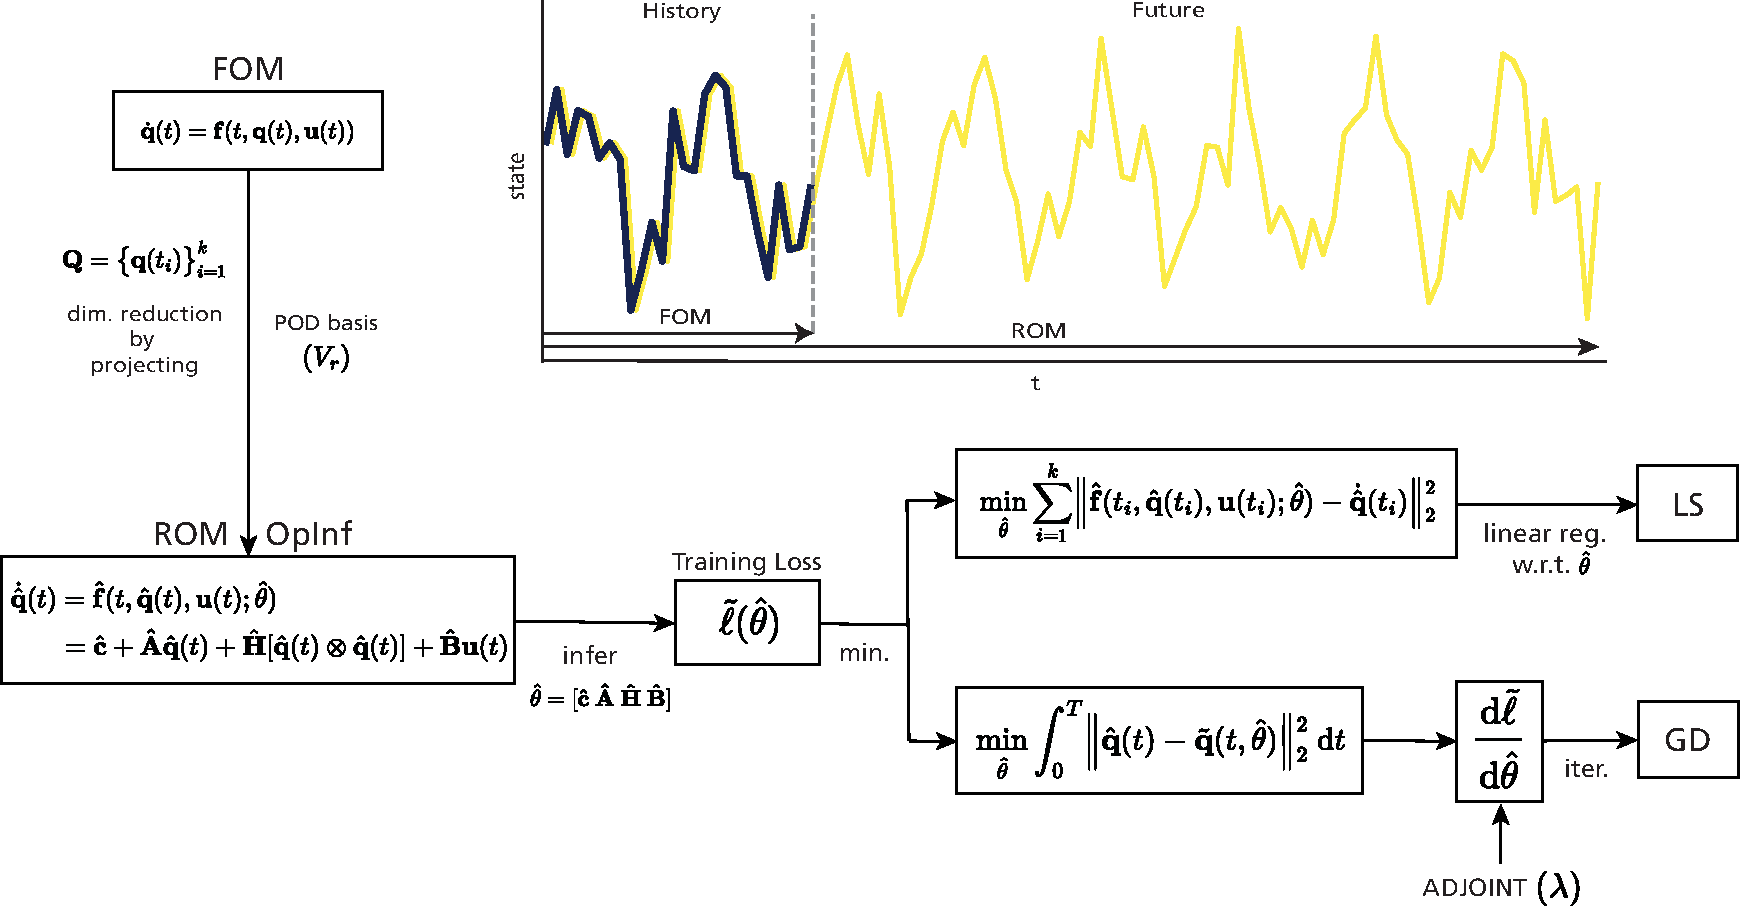
\includegraphics[width=.99\textwidth]{figures/intro_scheme.pdf}
    \caption{ROM inference process; OpInf (top branch) and adjoint method (bottom branch).}
    \label{fig:intro_rom1}
\end{figure}


%%%%%%%%%%%%%%%%%%%%%%%%%%%%%%%%%%%%%%%%%%%%%%%%%%%%%%%%%%%%%%%%%%%%%%%%%%%%%%%%%%%%%%%%%%

\newpage

\section{The Adjoint-State Equations}
\label{sec:adjoint_eqs}

\subsection*{Problem Setup}

For some given snapshot data, we consider their corresponding continuous interpolated true data $\hat{\mathbf{q}}_{\text{true}}(\cdot)$. We frame our loss minimization as an equality constraint optimization problem as in \cite{bradley2024pde}, i.e.,\\
\begin{align}
    \underset{\hat{\bm{\theta}}}{\mathrm{min}}~~\tilde\ell (\hat{\bm{\theta}})\equiv\underset{\hat{\bm{\theta}},\hat{\mathbf{q}}(\cdot)}{\mathrm{min}} ~~&\ell (\hat{\mathbf{q}}(\cdot))\notag\\
    \mathrm{s.t.}~~&\dot{\hat{\mathbf{q}}}(t) = \hat{\mathbf{f}}(\hat{\mathbf{q}}(t),\hat{\bm{\theta}}), \quad\hat{\mathbf{q}}(0)=\hat{\mathbf{q}}_0, \quad t\in[0,T],
    \label{eq:opt_problem}
\end{align}
where $\ell,~\tilde{\ell}$ are the loss functionals defined as in \eqref{eq:continuous_loss}, \eqref{eq:continuous_reduced_loss} and the constraint represents the ROM-OpInf as in \eqref{eq:redopinf}.

The associated Lagrangian to \eqref{eq:opt_problem} is defined as\\
\begin{equation}
        \mathscr{L}\bigl(\hat{\mathbf{q}}(\cdot),\hat{\bm{\theta}},\bm{\lambda}(\cdot)\bigr) \coloneqq \ell(\hat{\mathbf{q}}(\cdot)) - \int_0^T \bm{\lambda}(t)^{\top}\left( \dot{\hat{\mathbf{q}}}(t)-\hat{\mathbf{f}}(\hat{\mathbf{q}}(t),\hat{\bm{\theta}}) \right)\dd t - \bm{\lambda}(0)^{\top}(\hat{\mathbf{q}}(0)-\hat{\mathbf{q}}_0).
        \label{eq:lagrange_cost}
    \end{equation}
Since the constraints are satisfied for $\tilde{\mathbf{q}}(\cdot,\hat{\bm{\theta}})$, it follows\\
$$\mathscr{L}\bigl(\tilde{\mathbf{q}}(\cdot,\hat{\bm{\theta}}),\hat{\bm{\theta}}, \bm{\lambda}(\cdot)\bigr) = \tilde{\ell} (\hat{\bm{\theta}}).$$
In order to perform a gradient-based optimization process we need to compute\\
\begin{align*}
    \dv{\tilde{\ell}(\hat{\bm{\theta}})}{\hat{\bm{\theta}}} &= \dv{}{\hat{\bm{\theta}}} \mathscr{L}\bigl(\tilde{\mathbf{q}}(\cdot,\hat{\bm{\theta}}),\hat{\bm{\theta}},\bm{\lambda}(\cdot)\bigr) \\
    &= \dfrac{\partial\mathscr{L}}{\partial\hat{\bm{\theta}}} + \dfrac{\partial\mathscr{L}}{\partial\hat{\mathbf{q}}} \dfrac{\textrm{d}\tilde{\mathbf{q}}}{\textrm{d}\hat{\bm{\theta}}}\Bigg\vert_{\hat{\mathbf{q}}(\cdot) = \tilde{\mathbf{q}}(\cdot, \hat{\bm{\theta}} ) } \\
    &= 
  \frac{\partial\mathscr{L}}{\partial \hat{\bm{\theta}}}+
  \bm{D}_{\hat{\mathbf{q}}}\,\mathscr{L}\biggl(\tilde{\mathbf{q}}(\cdot,\hat{\bm{\theta}}),\,\hat{\bm{\theta}},\,\bm{\lambda}(\cdot);\,
    \dv{\tilde{\mathbf{q}}(\cdot,\hat{\bm{\theta}})}{\hat{\bm{\theta}}}
  \biggr).
\end{align*}
Then, we enforce stationarity of the derivative, $\dfrac{\partial\mathscr{L}}{\partial\hat{\mathbf{q}}} = \bm{0}$, condition that will provide the adjoint equations, ensuring\\
\begin{equation}
  \label{eq:equal_grad}
  \frac{\mathrm{d}\tilde{\ell}(\hat{\bm{\theta}})}{\mathrm{d}\hat{\bm{\theta}}}
  = \frac{\partial\mathscr{L}(\tilde{\mathbf{q}}(\cdot,\hat{\bm{\theta}})}{\partial\hat{\bm{\theta}}}.
\end{equation}

For such problem, the classical adjoint method as stated in \cite{bradley2024pde,luchini2024introduction} gives the following result.

\begin{theorem}[Adjoint method]
    \label{thm:adjoint_method}
    Assume $\hat{\mathbf{f}}$ and $g$ are continuously differentiable in both $\tilde{\mathbf{q}}$ and $\hat{\bm{\theta}}$ and that the initial state $\tilde{\mathbf{q}}(0)=\tilde{\mathbf{q}}_0$ is fixed (independent of $\hat{\bm{\theta}}$). The adjoint variable $\bm{\lambda}(t)\in\mathcal{C}^1(\mathcal{T})^r$ associated to a minimization problem such in \eqref{eq:opt_problem} satisfies a back propagation ODE\\ 
    \begin{equation}
        \dot{\bm{\lambda}}(t) = -\left[ \left(\dfrac{\partial \hat{\mathbf{f}}}{\partial\tilde{\mathbf{q}}}\right)^{\top}\bm{\lambda}(t) + \left( \dfrac{\partial g}{\partial \tilde{\mathbf{q}}} \right)^{\top} \right],\quad\bm{\lambda}(T)=\bm{0},
        \label{eq:adjoint_eqs}
    \end{equation}
    and the gradients w.r.t. the parameters of $\tilde\ell$ for the training loss\\
    \begin{equation*}
        \ell(\hat{\mathbf{q}}(\cdot)) \coloneqq \displaystyle\int_0^T g\bigl(\hat{\mathbf{q}}(t),t\bigr)~\dd t = \int_0^T \Bigl\|\hat{\mathbf{q}}(t) - \hat{\mathbf{q}}_{\mathrm{true}}(t)\Bigr\|_2^2~\dd t,
    \end{equation*}
    and the Lagrange cost ($\mathscr{L}$),\\
    \begin{equation*}
        \mathscr{L}\bigl(\tilde{\mathbf{q}}(\cdot,\hat{\bm{\theta}}),\hat{\bm{\theta}},\bm{\lambda}(\cdot)\bigr) \coloneqq \ell(\tilde{\mathbf{q}}(\cdot,\hat{\bm{\theta}})) - \int_0^T \bm{\lambda}(t)^{\top}\left( \dot{\tilde{\mathbf{q}}}(t,\hat{\bm{\theta}})-\hat{\mathbf{f}}(\tilde{\mathbf{q}},\hat{\bm{\theta}}) \right)\dd t - \bm{\lambda}(0)^{\top}(\tilde{\mathbf{q}}(0,\hat{\bm{\theta}})-\tilde{\mathbf{q}}_0),
        \label{eq:lagrange_cost2}
    \end{equation*}
    have the form\\
    \begin{equation}
        \frac{\mathrm{d}\tilde{\ell}(\hat{\bm{\theta}})}{\mathrm{d}\hat{\bm{\theta}}}
  = \frac{\partial\mathscr{L}(\tilde{\mathbf{q}}(\cdot,\hat{\bm{\theta}}))}{\partial\hat{\bm{\theta}}} = \int_0^T \bm{\lambda}(t)^{\top}\dfrac{\partial\hat{\mathbf{f}}(\tilde{\mathbf{q}},\hat{\bm{\theta}})}{\partial\hat{\bm{\theta}}}~\dd t.
        \label{eq:gradient_lagrange}
    \end{equation}
\end{theorem}

\subsection*{Proof (Lagrangian Formulation)}

Consider the  Lagrangian ($\mathscr{L}$) defined as\\
\begin{align*}
    \mathscr{L}(\tilde{\mathbf{q}}, \bm{\lambda},\hat{\bm{\theta}}) &\coloneqq \ell(\tilde{\mathbf{q}}(t,\hat{\bm{\theta}})) - \int_0^T \bm{\lambda}(t)^{\top}\left( \dot{\tilde{\mathbf{q}}}(t,\hat{\bm{\theta}}) - \hat{\mathbf{f}}(\tilde{\mathbf{q}}(t,\hat{\bm{\theta}}),\hat{\bm{\theta}})  \right)\dd t -\bm{\lambda}(0)^{\top}(\tilde{\mathbf{q}}(0,\hat{\bm{\theta}})-\tilde{\mathbf{q}}_0)\\
    &= \int_0^T \left( g(\tilde{\mathbf{q}}(t,\hat{\bm{\theta}}),t) - \bm{\lambda}(t)^{\top}\left( \dot{\tilde{\mathbf{q}}}(t) - \hat{\mathbf{f}}(\tilde{\mathbf{q}}(t,\hat{\bm{\theta}}),\hat{\bm{\theta}})  \right) \right)\dd t-\bm{\lambda}(0)^{\top}(\tilde{\mathbf{q}}(0,\hat{\bm{\theta}})-\tilde{\mathbf{q}}_0).
\end{align*}
Differentiating the Lagrangian w.r.t. $\hat{\bm{\theta}}$, we have\\
\begin{align*}
    \pdv{\mathscr{L}}{\hat{\bm{\theta}}} &= \int_0^T\left[ \pdv{g}{\hat{\bm{\theta}}} + \pdv{g}{\tilde{\mathbf{q}}} \dv{\tilde{\mathbf{q}}}{\hat{\bm{\theta}}} - \bm{\lambda}(t)^{\top} \left( \dv{t}\dv{\tilde{\mathbf{q}}}{\hat{\bm{\theta}}} - \pdv{\hat{\mathbf{f}}}{\hat{\bm{\theta}}} - \pdv{\hat{\mathbf{f}}}{\tilde{\mathbf{q}}}\dv{\tilde{\mathbf{q}}}{\hat{\bm{\theta}}} \right) \right]\dd t - \bm{\lambda}(0)^{\top}\dv{\tilde{\mathbf{q}}}{\hat{\bm{\theta}}}~(0)\notag\\
    &= \int_0^T \left[\pdv{g}{\hat{\bm{\theta}}} + \bm{\lambda}(t)^{\top} \pdv{\hat{\mathbf{f}}}{\hat{\bm{\theta}}}+ \left( \pdv{g}{\tilde{\mathbf{q}}} + \bm{\lambda}(t)^{\top}\pdv{\hat{\mathbf{f}}}{\tilde{\mathbf{q}}}-\bm{\lambda}(t)^{\top}\dv{t} \right)\dv{\tilde{\mathbf{q}}}{\hat{\bm{\theta}}} \right]\dd t- \bm{\lambda}(0)^{\top}\dv{\tilde{\mathbf{q}}}{\hat{\bm{\theta}}}~(0). 
\end{align*}
In order to avoid the computation of $\mathrm{d}{\tilde{\mathbf{q}}}/\mathrm{d}{\hat{\bm{\theta}}}$, i.e., the sensitity of the trajectory w.r.t. the parameters, which can be extremely hard, we apply a change of variables (adjoint method). Integrating by parts, we get rid of $\displaystyle\dv{t}\dv{\tilde{\mathbf{q}}}{\hat{\bm{\theta}}}$ in the last part of the above integral,\\
\begin{align*}
    \int_0^T -\bm{\lambda}(t)^{\top}\dv{t}\dv{\tilde{\mathbf{q}}}{\hat{\bm{\theta}}}~\dd t &= \left[ -\bm{\lambda}(t)^{\top}\dv{\tilde{\mathbf{q}}}{\hat{\bm{\theta}}}\right]_0^T + \int_0^T \left( \dv{\bm{\lambda}}{t}\right)^{\top}\dv{\tilde{\mathbf{q}}}{\hat{\bm{\theta}}}~\dd t\\
    &= \bm{\lambda}(0)^{\top}\dv{\tilde{\mathbf{q}}}{\hat{\bm{\theta}}}~(0) - \bm{\lambda}(T)^{\top}\dv{\tilde{\mathbf{q}}}{\hat{\bm{\theta}}}~(T) + \int_0^T \left( \dv{\bm{\lambda}}{t}\right)^{\top}\dv{\tilde{\mathbf{q}}}{\hat{\bm{\theta}}}~\dd t.
\end{align*}
Plugin this expression, the Lagrangian sensitivity equation  yields\\
\begin{align*}
   \pdv{\mathscr{L}}{\hat{\bm{\theta}}} &= \int_0^T\left[ \pdv{g}{\hat{\bm{\theta}}} + \bm{\lambda}(t)^{\top} \pdv{\hat{\mathbf{f}}}{\hat{\bm{\theta}}} + \underbrace{\left( \pdv{g}{\tilde{\mathbf{q}}} + \bm{\lambda}(t)^{\top}\pdv{\hat{\mathbf{f}}}{\tilde{\mathbf{q}}}+ \dot{\bm{\lambda}}(t)^{\top}\right)}_{\text{make = 0}} \dv{\tilde{\mathbf{q}}}{\hat{\bm{\theta}}} \right]\dd t \\
   & - \bm{\lambda}(0)^{\top}\dv{\tilde{\mathbf{q}}}{\hat{\bm{\theta}}}~(0)+\bm{\lambda}(0)^{\top}\dv{\tilde{\mathbf{q}}}{\hat{\bm{\theta}}}~(0) - \underbrace{\bm{\lambda}(T)^{\top}\dv{\tilde{\mathbf{q}}}{\hat{\bm{\theta}}}~(T)}_{\text{make = 0}}.
\end{align*}
We recognize all the terms multiplying the sensitivity $\displaystyle\dv{\tilde{\mathbf{q}}}{\hat{\bm{\theta}}}$ as the expression $\displaystyle\pdv{\mathscr{L}}{\tilde{\mathbf{q}}}$ which we make zero together with $\bm{\lambda}(T)$, since $\bm{\lambda}$ arbitrary.
 After transposing and rearranging terms, we obtain the desired adjoint equations\\
\begin{equation*}
    \dot{\bm{\lambda}}(t) = -\left[ \left(\pdv{\hat{\mathbf{f}}}{\tilde{\mathbf{q}}}\right)^{\top} \bm{\lambda}(t)  + \left(\pdv{g}{\tilde{\mathbf{q}}}\right)^{\top}\right], \quad\bm{\lambda}(T) = \bm{0}.
\end{equation*}
By construction, as we have shown in the problem setup,  minimizing the Lagrangian $\mathscr{L}$ is the same as minimizing the loss functional $\tilde\ell$ since\\
$$\pdv{\mathscr{L}}{\hat{\bm{\theta}}} = \dv{\tilde\ell}{\hat{\bm{\theta}}}.$$
By definition, $g$ is not dependent on $\hat{\bm{\theta}}$ which implies that $\displaystyle\pdv{g}{\hat{\bm{\theta}}}=\bm{0}$. Hence, the final expression for the gradients yields\\
\begin{equation*}
    \pdv{\mathscr{L}}{\hat{\bm{\theta}}} =\dv{\tilde\ell}{\hat{\bm{\theta}}} = \int_0^T \bm{\lambda}(t)^{\top} \pdv{\hat{\mathbf{f}}}{\hat{\bm{\theta}}}~\dd t.
\end{equation*}
This completes the proof.
\qed

\subsection*{Formulation for the Quadratic Form}

We now consider the previously stated OpInf quadratic form in \eqref{eq:fompoly} to derive the adjoint equations for that specific problem. This derivation was inspired by the notes of \cite{mcquarrie2024bayesian}. For convenience, we write the constraint equation as\\ 
$$\boldsymbol{c}(\hat{\mathbf{q}}(t),\hat{\bm{\theta}}) \coloneqq \dot{\hat{\mathbf{q}}}(t) - \hat{\mathbf{c}} - \hat{\mathbf{A}}\hat{\mathbf{q}}(t) - \hat{\mathbf{H}}[\hat{\mathbf{q}}(t)\otimes \hat{\mathbf{q}}(t)] - \hat{\mathbf{B}}\mathbf{u}.$$
Here, $\hat{\mathbf{H}}\in \mathbb{R}^{r\times r^2}$ is Kronecker-symmetric, i.e., $\hat{\mathbf{H}}[\hat{\mathbf{q}}\otimes \mathbf{v}] = \hat{\mathbf{H}}[\mathbf{v}\otimes \hat{\mathbf{q}}]$. Then, the Lagrangian (objective - adjoint $\times$ constraint - adjoint(0) $\times$ initial condition) can be rewritten as\\
\begin{align*}
    \mathscr{L}(\hat{\mathbf{q}}, \bm{\lambda}; \hat{\bm{\theta}}) &= \ell(\hat{\mathbf{q}}(t)) - \int_0^T \bm{\lambda}(t)^{\top}\boldsymbol{c}(\hat{\mathbf{q}}(t),\hat{\bm{\theta}})~\mathrm{d}t - \bm{\lambda}(0)^{\top}(\hat{\mathbf{q}}(0)-\hat{\mathbf{q}}_0)\\
    &= \int_0^T g\bigl(\hat{\mathbf{q}}(t),t \bigl)~\mathrm{d}t \\
    &- \int_0^T \bm{\lambda}(t)^{\top}\bigl(\dot{\hat{\mathbf{q}}}(t) - \hat{\mathbf{c}} - \hat{\mathbf{A}}\hat{\mathbf{q}}(t) - \hat{\mathbf{H}}(\hat{\mathbf{q}}(t)\otimes \hat{\mathbf{q}}(t)) - \hat{\mathbf{B}}\mathbf{u}\bigr)~\mathrm{d}t \\
    &-\bm{\lambda}(0)^{\top}(\hat{\mathbf{q}}(0)-\hat{\mathbf{q}}_0),
\end{align*}
where the adjoint variable $\bm{\lambda}\in\mathcal{C}^1(\mathcal{T})^r$ has the same size as the state variable $\hat{\mathbf{q}}$. The adjoint equation for $\bm{\lambda}(t)$ is derived by setting\\
$$ \bm{D}_{\hat{\mathbf{q}}} \mathscr{L}(\hat{\mathbf{q}},\bm{\lambda,\hat{\bm{\theta}}};\mathbf{v}) = \dv{}{\varepsilon}[\mathscr{L}(\hat{\mathbf{q}}+\varepsilon \mathbf{v},\bm{\lambda,\hat{\bm{\theta}}})]_{\varepsilon=0} = \bm{0}~~~\forall~\mathbf{v}\in\mathcal{C}^1(\mathcal{T})^r,$$a directional (Gâteaux) derivative. Noting first that\\
\begin{align*}
    \dv{}{\varepsilon}[\mathcal{\ell}(\hat{\mathbf{q}}+\varepsilon \mathbf{v},\hat{\bm{\theta}})]_{\varepsilon=0} &= \int_0^T \dv{}{\varepsilon}[g(\hat{\mathbf{q}}(t)+\varepsilon \mathbf{v}(t),t)]_{\varepsilon=0}~\mathrm{d}t = \int_0^T \nabla_{\hat{\mathbf{q}}}~g(\hat{\mathbf{q}}(t),t)^{\top}\mathbf{v}(t)~\mathrm{d}t,\\
    \dv{}{\varepsilon}[\boldsymbol{c}(\hat{\mathbf{q}}+\varepsilon \mathbf{v},\hat{\bm{\theta}})]_{\varepsilon=0} &= \dot{\mathbf{v}}(t) - \hat{\mathbf{A}}\mathbf{v}(t) - 2\hat{\mathbf{H}}[\hat{\mathbf{q}}(t)\otimes \mathbf{v}(t)],
\end{align*}
the adjoint equations are given by\\
\begin{align*}
    \bm{0} &= \int_0^T \nabla_{\hat{\mathbf{q}}}~g(\hat{\mathbf{q}}(t),t)^{\top}\mathbf{v}(t)~\mathrm{d}t\\
    &- \int_0^T \bm{\lambda}(t)^{\top} \left( \dot{\mathbf{v}}(t) - \hat{\mathbf{A}}\mathbf{v}(t) - 2\hat{\mathbf{H}}[\hat{\mathbf{q}}(t)\otimes \mathbf{v}(t)] \right)~\mathrm{d}t~- \bm{\lambda}(0)^{\top}\mathbf{v}(0). 
\end{align*}
We want to write these adjoint equations as a weak form with test function $\mathbf{v}$. Integration by parts yields\\
\begin{align*}
    -\int_0^T\bm{\lambda}(t)^{\top} \dot{\mathbf{v}}(t)~\mathrm{d}t &= -\left[ \bm{\lambda}(t)^{\top} \mathbf{v}(t) \right]_0^T + \int_0^T \dot{\bm{\lambda}}(t)^{\top}\mathbf{v}(t)~\mathrm{d}t\\
    &= \bm{\lambda}(0)^{\top} \mathbf{v}(0) - \bm{\lambda}(T)^{\top} \mathbf{v}(T) + \int_0^T \mathbf{v}(t)^{\top}\dot{\bm{\lambda}}(t)~\mathrm{d}t.
\end{align*}
Using this identity and transposing each (scalar) term, the adjoint equations become\\
\begin{equation*}
    \bm{0} = \int_0^T \mathbf{v}(t)^{\top} \left( \dot{\bm{\lambda}}(t) + \hat{\mathbf{A}}^{\top} \bm{\lambda}(t) + 2\tilde{\mathbf{H}}[\hat{\mathbf{q}}(t)\otimes \bm{\lambda}(t)] + \nabla_{\hat{\mathbf{q}}}~g(\hat{\mathbf{q}}(t),t) \right)\mathrm{d}t - \mathbf{v}(T)^{\top}\bm{\lambda}(T), 
\end{equation*}
where $\tilde{\mathbf{H}}\in\mathbb{R}^{r\times r^2}$ is the matrix such that\\
$$\bm{\lambda}^{\top}\hat{\mathbf{H}}[\hat{\mathbf{q}}\otimes \mathbf{v}] = \mathbf{v}^{\top}\tilde{\mathbf{H}}[\hat{\mathbf{q}}\otimes \bm{\lambda}],~~~\forall~\hat{\mathbf{q}}, \mathbf{v}, \bm{\lambda} \in \mathbb{R}^r.$$
Since $\mathbf{v}$ is arbitrary, we recognize the above expression as a weak form with corresponding strong form\\
\begin{equation*}
    -\dot{\bm{\lambda}}(t) = \hat{\mathbf{A}}^{\top} \bm{\lambda}(t) + 2\tilde{\mathbf{H}}[\hat{\mathbf{q}}(t)\otimes \bm{\lambda}(t)] + \nabla_{\hat{\mathbf{q}}}~g(\hat{\mathbf{q}}(t),t),~~~\bm{\lambda}(T)=\bm{0},\quad t\in [0,T].
\end{equation*}
This linear (but non-autonomous) system can be solved with `backward time-integration' given a trajectory $\hat{\mathbf{q}}(t)$. The system can be written in a more clearly linear form (with respect to $\bm{\lambda}(t)$) as\\
\begin{align}
    \label{eq:gradient_fq}
     \dot{\bm{\lambda}}(t) &= -\left(\hat{\mathbf{A}}^{\top} + 2\mathbf{M}(\hat{\mathbf{q}}(t))\right)\bm{\lambda}(t) - \nabla_{\hat{\mathbf{q}}}~g(\hat{\mathbf{q}}(t),t),\notag\\
    &~\hspace{8.8cm}~~~~~\bm{\lambda}(T)=\bm{0},\\
    &= -\nabla_{\hat{\mathbf{q}}}~\hat{\mathbf{f}}(\hat{\mathbf{q}}(t),\hat{\bm{\theta}})\bm{\lambda}(t) - \nabla_{\hat{\mathbf{q}}}~g(\hat{\mathbf{q}}(t),t)\notag,
\end{align}
where $\mathbf{M}(\hat{\mathbf{q}}(t))\in\mathbb{R}^{r\times r}$ is the matrix such that\\
\begin{equation*}
    \mathbf{M}(\hat{\mathbf{q}}(t)) \bm{\lambda} = \tilde{\mathbf{H}}[\hat{\mathbf{q}}(t)\otimes \bm{\lambda}(t)].
\end{equation*}
We defer the computation of $\nabla_{\hat{\mathbf{q}}}~g$, along with the remaining gradients needed for the adjoint method, to Section~\ref{sec:four_gradients}.



%%%%%%

\subsection*{Alternative Proof (Sensitivity Analysis of the Primal Problem)}

We start from the \emph{primal} sensitivity equations for the state $\hat{\mathbf{q}}(t)$ and parameters $\hat{\theta}_i$ for $i=1,\dots,d$:\\
$$\dot{\hat{\mathbf{q}}}(t)
= \hat{\mathbf{f}}\bigl(\hat{\mathbf{q}}(t),\hat{\bm{\theta}}\bigr),
\qquad
\partial_{\hat{\theta}_i}\dot{\hat{\mathbf{q}}}(t)
= \frac{\partial \hat{\mathbf{f}}}{\partial \hat{\mathbf{q}}}
  \bigl(\hat{\mathbf{q}}(t),\hat{\bm{\theta}}\bigr)^{\!\top}
  \,\partial_{\hat{\theta}_i}\hat{\mathbf{q}}(t)
+ \partial_{\hat{\theta}_i}\hat{\mathbf{f}}
  \bigl(\hat{\mathbf{q}}(t),\hat{\bm{\theta}}\bigr).$$
Multiplying the second equation by an arbitrary test function $\mathbf{v}(\cdot)\in\mathcal{C}^1(\mathcal{T})^r$, integrating from $0$ to $T$, and rearranging, we can rewrite the primal problem in its weak form\\
$$\int_{0}^{T}
\Biggl[
  \partial_{\hat{\theta}_i}\dot{\hat{\mathbf{q}}}(t)
  - \biggl(\dfrac{\partial \hat{\mathbf{f}}}{\partial \hat{\mathbf{q}}}\biggr)^{\top}\,
    \partial_{\hat{\theta}_i}\hat{\mathbf{q}}(t)
\Biggr]^{\!\top}
\mathbf{v}(t)\,\mathrm{d}t
=
\int_{0}^{T}
\bigl(\partial_{\hat{\theta}_i}\hat{\mathbf{f}}\bigr)^{\!\top}
\mathbf{v}(t)\,\mathrm{d}t,$$
or, in operator notation,\\
$$\langle \mathcal{L}\,\partial_{\hat{\theta}_i}\hat{\mathbf{q}},\,\mathbf{v}\rangle
= \langle \partial_{\hat{\theta}_i}\hat{\mathbf{f}},\,\mathbf{v}\rangle,$$
where the operator\\
$$ \mathcal{L}: \mathcal{C}^1(\mathcal{T})^r\to\mathcal{C}^0(\mathcal{T})^r,$$ 
with both domain and codomain equipped with the usual $L^2$-inner product, is given by\\
$$(\mathcal{L}\mathbf{w})(t) = \dot{\mathbf{w}}(t) - \biggl(\dfrac{\partial \hat{\mathbf{f}}}{\partial \hat{\mathbf{q}}}\biggr)^{\top}\mathbf{w}(t),$$
for any $\mathbf{w}(\cdot)\in\mathcal{C}^1(\mathcal{T})^r$. 

On the other hand, the gradient of the loss $\tilde{\ell}$ with respect to $\hat{\theta}_i$ is\\
$$\frac{\mathrm{d}}{\mathrm{d}\hat{\theta}_i}\,\tilde\ell
= \int_{0}^{T}
\frac{\partial g}{\partial \hat{\mathbf{q}}}\bigl(\hat{\mathbf{q}}(t),t\bigr)^{\!\top}
\,\partial_{\hat{\theta}_i}\hat{\mathbf{q}}(t)\,\mathrm{d}t
= \langle \nabla_{\hat{\mathbf{q}}}\,g,\,\partial_{\hat{\theta}_i}\hat{\mathbf{q}}\rangle.$$
Now, we define the adjoint problem by introducing an adjoint variable $\bm{\lambda}(\cdot)\in\mathcal{C}^1(\mathcal{T})^r$ such that\\
$$\langle \mathbf{w},\,\tilde{\mathcal{L}}\,\bm{\lambda}\rangle
= \langle \nabla_{\hat{\mathbf{q}}}\,g,\,\mathbf{w}\rangle
\quad\forall\,\mathbf{w}(\cdot)\in\mathcal{C}^1(\mathcal{T})^r\text{ with }\mathbf{w}(0)=\bm{0},$$
where $\tilde{\mathcal{L}}$ is the adjoint of $\mathcal{L}$.  By the definition of the adjoint operator this is equivalent to\\
$$\langle \mathcal{L}\,\mathbf{w},\,\bm{\lambda}\rangle
= \langle \nabla_{\hat{\mathbf{q}}}\,g,\,\mathbf{w}\rangle.$$
Choosing $\mathbf{w} = \partial_{\hat{\theta}_i}\hat{\mathbf{q}}$ in this identity immediately gives\\
$$\frac{\dd}{\dd\hat{\theta}_i}\,\tilde\ell
= \bigl\langle \mathcal{L}\,\partial_{\hat{\theta}_i}\hat{\mathbf{q}},\,\bm{\lambda}\bigr\rangle
\underset{
  \substack{
    \text{primal problem}\\
    \text{with }\mathbf{v}\,=\,\bm{\lambda}
  }
}{=}
\bigl\langle \partial_{\hat{\theta}_i}\hat{\mathbf{f}},\,\bm{\lambda}\bigr\rangle
= \int_{0}^{T}
  \bm{\lambda}(t)^{\!\top}\,
  \partial_{\hat{\theta}_i}\hat{\mathbf{f}}(t)\,
  \dd t.$$
To derive the adjoint ODE itself, we expand\\
$$\langle \mathcal{L}\,\mathbf{w},\,\bm{\lambda}\rangle
= \int_{0}^{T}
\Biggl[
  \dot{\mathbf{w}}(t)
  - \biggl(\dfrac{\partial\hat{\mathbf{f}}}{\partial\hat{\mathbf{q}}}\biggr)^{\!\top}
    \mathbf{w}(t)
\Biggr]^{\!\top}
\bm{\lambda}(t)\,\mathrm{d}t
= \int_{0}^{T}
\biggl(\dfrac{\partial g}{\partial\hat{\mathbf{q}}}\biggr)^{\!\top}
\mathbf{w}(t)\,\mathrm{d}t = \langle \nabla_{\hat{\mathbf{q}}}\,g,\,\mathbf{w}\rangle.$$
Integrating by parts the term\\
$$\int_{0}^{T}\dot{\mathbf{w}}(t)^{\!\top}\bm{\lambda}(t)\,\dd t =  \left[ \mathbf{w}(t)^{\top}\bm{\lambda}(t)\right]_0^T - \int_0^T \dot{\bm{\lambda}}(t)^{\top}\cdot\mathbf{w}(t)~\dd t,$$
using $\mathbf{w}(0)=\bm{0}$ and imposing the natural terminal condition $\bm{\lambda}(T)=\bm{0}$ to kill the boundary term, we obtain\\
$$\int_{0}^{T}
\bigl[
  -\,\dot{\bm{\lambda}}(t)
\bigr]^{\!\top}
\mathbf{w}(t)\,\mathrm{d}t
=
\int_{0}^{T}
\Biggl[
  \biggl(\dfrac{\partial\hat{\mathbf{f}}}{\partial\hat{\mathbf{q}}}\biggr)^{\!\top}\bm{\lambda}(t)
  + \biggl(\dfrac{\partial g}{\partial\hat{\mathbf{q}}}\biggr)^{\!\top}
\Biggr]^{\!\top}
\mathbf{w}(t)\,\mathrm{d}t.$$
Since $\mathbf{w}$ is arbitrary, the integrands coincide, yielding the final expression for the adjoint equations\\
$$\dot{\bm{\lambda}}(t)
= -\Biggl[
    \biggl(\dfrac{\partial\hat{\mathbf{f}}}{\partial\hat{\mathbf{q}}}\biggr)^{\!\top}\bm{\lambda}(t)
    + \biggl(\dfrac{\partial g}{\partial\hat{\mathbf{q}}}\biggr)^{\!\top}
  \Biggr],
\quad
\bm{\lambda}(T)=\bm{0}.$$
\qed

\noindent\textbf{Remark.} While the adjoint equations are independent of $i=1,\dots, d$, i.e., the size of the $\hat{\bm{\theta}}$ parameters, the primal sensitivity equations require solving $d$ systems for $\displaystyle\{\partial_{\hat{\theta}_i} \dot{\hat{\mathbf{q}}}(t)\}_{i=1}^d$, making the adjoint method particularly advantageous to the primal when $d \gg 1$.

%%%%%%

\subsection*{Theoretical Validation}

One question that arises at this point is whether the solution provided by the adjoint method $\bm{\lambda}(t)$, obtained by solving the backward propagation ODE, is indeed correct and reliable for guiding the optimization of $\hat{\bm{\theta}}$. To address this, we present both theoretical and possible empirical verification arguments in support of the adjoint approach.

The correctness of the adjoint method follows from three fundamental principles of mathematical optimization:

\begin{itemize}
    \item \textbf{Optimality Conditions.}  The adjoint equations emerge directly from the Karush-Kuhn-Tucker (KKT) conditions for constrained optimization \cite{nocedal1999numerical}. By forming the Lagrangian\\
    $$\mathscr{L}(\hat{\mathbf{q}}, \bm{\lambda}, \hat{\bm{\theta}}) 
    = \int_{t_0}^{t_f} g(\hat{\mathbf{q}}(t),t) \,\mathrm{d}t
      - \int_{t_0}^{t_f} \bm{\lambda}(t)^\top \bigl[\dot{\hat{\mathbf{q}}}(t)-\hat{\mathbf{f}}(\hat{\mathbf{q}}(t),\hat{\bm{\theta}})\bigr]\,\mathrm{d}t
      - \bm{\lambda}(t_0)^\top \bigl(\hat{\mathbf{q}}(t_0)-\hat{\mathbf{q}}_0\bigr) ,$$
  the first-order stationarity conditions with respect to~$\hat{\mathbf{q}}$ yield the adjoint ODE that ensures the computed gradients respect the dynamical constraints.
    
    \item \textbf{Duality}: The adjoint variable $\bm{\lambda}(t)$ has a fundamental interpretation as sensitivity measure. Specifically, it quantifies how perturbations in the state vector $\hat{\mathbf{q}}(t)$ propagate through the system to affect the final loss. This duality perspective aligns with reverse-mode automatic differentiation in machine learning \cite{chen2018neural}, where gradients flow backward through computational graphs.

    \item \textbf{Consistency with Pontryagin's Maximum Principle.}  Defining the Hamiltonian\\
  $$\mathcal{H}(\hat{\mathbf{q}}, \bm{\lambda}, \hat{\bm{\theta}}) 
      = \bm{\lambda}^\top \hat{\mathbf{f}}(\hat{\mathbf{q}}, \hat{\bm{\theta}}) 
      + g(\hat{\mathbf{q}}, t),$$
  Pontryagin's principle prescribes the costate equation\\
  $$\dot{\bm{\lambda}}(t) 
      = - \left(\frac{\partial \mathcal{H}}{\partial \hat{\mathbf{q}}} \right)^{\top}
      = - \left(\frac{\partial \hat{\mathbf{f}}}{\partial \hat{\mathbf{q}}} \right)^{\top}\bm{\lambda}(t) -  \left(\frac{\partial g}{\partial \hat{\mathbf{q}}} \right)^{\top}.$$
  The adjoint method exactly recovers these necessary conditions for optimality in control theory \cite{liberzon2011calculus}.
\end{itemize}

In conclusion, the adjoint method computes the costate $\bm{\lambda}(t)$ by rigorously enforcing the first-order optimality conditions of the Lagrangian in a dynamical setting. Its theoretical basis in the Karush-Kuhn-Tucker framework, duality interpretation, and alignment with Pontryagin's principle ensures that the resulting gradients are exact up to numerical precision. Coupled with empirical validation strategies such as finite-difference gradient checking, convergence monitoring, and assessment of physical plausibility, the adjoint method provides a reliable and accurate mechanism for optimizing parameters in dynamical systems.

%%%%%%%%%%%%%%%%%%%%%%%%%%%%%%%%%%%%%%%%%%%%%%%%%%%%%%%%%%%%%%%%%%%%%%%%%%%%%%%%%%%%%%%%

\section{Equations of the Three Gradients}
\label{sec:four_gradients}

Note that the adjoint method used here requires computing the following three gradients:\\
$$\pdv{\hat{\mathbf{f}}}{\hat{\mathbf{q}}},  \quad \pdv{g}{\hat{\mathbf{q}}}, \quad \text{and} \quad \pdv{\hat{\mathbf{f}}}{\hat{\bm{\theta}}},$$
where\\
$$\hat{\mathbf{f}}:\mathbb{R}^r \times \mathbb{R}^d \to \mathbb{R}^r$$ 
denotes the right-hand side of the reduced-order model (ROM-OpInf) dynamics, and\\
$$g:\mathbb{R}^r\times [0,T]\to \mathbb{R}$$ 
defines the integrand of the loss functional $\ell$. The efficient computation of these gradients is crucial for both the backward integration of the adjoint equation and for evaluating the total derivative of the reduced loss $\tilde\ell$. What follows is a detailed derivation of the expressions of each of these gradients.

\subsection{$\bm{\nabla}_{\hat{\mathbf{q}}}~\hat{\mathbf{f}}\bigl(\hat{\mathbf{q}}(t), \hat{\bm{\theta}}\bigr)$}

We begin by recalling the definition:\\
$$
\hat{\mathbf{f}}(\hat{\mathbf{q}}(t), \hat{\bm{\theta}}) = \hat{\mathbf{c}} + \hat{\mathbf{A}}\hat{\mathbf{q}}(t) + \hat{\mathbf{H}}\bigl( \hat{\mathbf{q}}(t)\otimes \hat{\mathbf{q}}(t) \bigr) + \hat{\mathbf{B}}\mathbf{u}(t).
$$
To compute the derivative of $\hat{\mathbf{f}}$ with respect to $\hat{\mathbf{q}}$, we consider the Gâteaux derivative in the direction of an arbitrary vector $\mathbf{v}\in \mathbb{R}^r$:\\
$$
\bm{D}_{\hat{\mathbf{q}}}~\hat{\mathbf{f}}(\hat{\mathbf{q}}, \hat{\bm{\theta}}; \mathbf{v}) = \bm{D}_{\hat{\mathbf{q}}}~\hat{\mathbf{f}}[\mathbf{v}] = \lim_{\varepsilon \to 0} \frac{\hat{\mathbf{f}}(\hat{\mathbf{q}} + \varepsilon \mathbf{v}, \hat{\bm{\theta}}) - \hat{\mathbf{f}}(\hat{\mathbf{q}}, \hat{\bm{\theta}})}{\varepsilon} = \dv{}{\varepsilon} \left[ \hat{\mathbf{f}}(\hat{\mathbf{q}} + \varepsilon \mathbf{v}, \hat{\bm{\theta}}) \right]_{\varepsilon = 0}.
$$
Expanding the function $\hat{\mathbf{f}}$ at $\hat{\mathbf{q}} + \varepsilon \mathbf{v}$, we obtain:\\
$$
\hat{\mathbf{f}}(\hat{\mathbf{q}} + \varepsilon \mathbf{v}, \hat{\bm{\theta}}) = \hat{\mathbf{c}} + \hat{\mathbf{A}}(\hat{\mathbf{q}} + \varepsilon \mathbf{v}) + \hat{\mathbf{H}}\bigl( (\hat{\mathbf{q}} + \varepsilon \mathbf{v}) \otimes (\hat{\mathbf{q}} + \varepsilon \mathbf{v}) \bigr) + \hat{\mathbf{B}}\mathbf{u}(t).
$$
The quadratic term expands as:\\
$$
(\hat{\mathbf{q}} + \varepsilon \mathbf{v}) \otimes (\hat{\mathbf{q}} + \varepsilon \mathbf{v}) = \hat{\mathbf{q}} \otimes \hat{\mathbf{q}} + \varepsilon (\hat{\mathbf{q}} \otimes \mathbf{v} + \mathbf{v} \otimes \hat{\mathbf{q}}) + \varepsilon^2 (\mathbf{v} \otimes \mathbf{v}).
$$
Substituting back into the expression for $\hat{\mathbf{f}}$, we get:\\
$$
\hat{\mathbf{f}}(\hat{\mathbf{q}} + \varepsilon \mathbf{v}, \hat{\bm{\theta}}) = \hat{\mathbf{c}} + \hat{\mathbf{A}}\hat{\mathbf{q}} + \varepsilon \hat{\mathbf{A}}\mathbf{v} + \hat{\mathbf{H}}(\hat{\mathbf{q}} \otimes \hat{\mathbf{q}}) + \varepsilon \hat{\mathbf{H}}(\hat{\mathbf{q}} \otimes \mathbf{v} + \mathbf{v} \otimes \hat{\mathbf{q}}) + \hat{\mathbf{B}}\mathbf{u}(t) + \mathcal{O}(\varepsilon^2).
$$
Differentiating with respect to $\varepsilon$ and evaluating at $\varepsilon = 0$ yields:\\
$$
\bm{D}_{\hat{\mathbf{q}}}~\hat{\mathbf{f}}[\mathbf{v}] = \hat{\mathbf{A}}\mathbf{v} + 2\hat{\mathbf{H}}(\hat{\mathbf{q}} \otimes \mathbf{v}),
$$
where we use the fact that $\hat{\mathbf{H}}$ is Kronecker symmetric, i.e., $\hat{\mathbf{H}}(\hat{\mathbf{q}} \otimes \mathbf{v}) = \hat{\mathbf{H}}(\mathbf{v} \otimes \hat{\mathbf{q}})$.
To express this as a gradient under the $L^2$ inner product, we match directional derivatives with inner products:\\
$$
\left( \hat{\mathbf{A}} + 2\hat{\mathbf{H}}\bigl( \hat{\mathbf{q}} \otimes \mathbf{I}_r \bigr) \right) \mathbf{v} = \bm{D}_{\hat{\mathbf{q}}}~\hat{\mathbf{f}}[\mathbf{v}] = \langle \nabla_{\hat{\mathbf{q}}}~\hat{\mathbf{f}},\;\mathbf{v} \rangle = \left( \nabla_{\hat{\mathbf{q}}}~\hat{\mathbf{f}} \right)^{\top}  \mathbf{v},
$$
where $\mathbf{I}_r$ is the identity matrix of size $r$. Therefore, the gradient is given by:\\
\begin{equation}
    \nabla_{\hat{\mathbf{q}}}~\hat{\mathbf{f}}(\hat{\mathbf{q}}, \hat{\bm{\theta}}) = \hat{\mathbf{A}}^{\top} + \left( 2\hat{\mathbf{H}}\bigl( \hat{\mathbf{q}} \otimes \mathbf{I}_r \bigr) \right)^{\top} = \hat{\mathbf{A}}^{\top} + 2\mathbf{M}(\hat{\mathbf{q}}) ~~ \in \mathbb{R}^{r \times r},
    \label{eq:gradient_1}
\end{equation}
where we define $\mathbf{M}(\hat{\mathbf{q}}(t)) := \left( \hat{\mathbf{H}}( \hat{\mathbf{q}}(t) \otimes \mathbf{I}_r ) \right)^{\top} \in \mathbb{R}^{r \times r}$.

Note that this result is consistent with the formulation presented in the first proof example, which concerns the quadratic form \eqref{eq:gradient_fq}.


\subsection{$\bm{\nabla}_{\hat{\mathbf{q}}}\,g\bigl(\hat{\mathbf{q}}(t),t\bigr)$}

By definition, the loss integrand is given by\\
$$g\bigl(\hat{\mathbf{q}},t\bigr)= \Bigl\|\hat{\mathbf{q}}(t) - \hat{\mathbf{q}}_{\mathrm{true}}(t)\Bigr\|_2^2\,,$$
where $\hat{\mathbf{q}}(t)$ denotes the predicted state vector at time $t$, and $\hat{\mathbf{q}}_{\text{true}}(t)$ is the corresponding true data state vector at the same time point.
We introduce, for convenience, the residual\\
$$\mathbf{r}(\hat{\mathbf{q}},t):=  \hat{\mathbf{q}}(t) - \hat{\mathbf{q}}_{\mathrm{true}}(t).$$
Then, the Gateaux derivative of $g$ in the direction $\mathbf{v}\in\mathbb{R}^r$ is\\
\begin{align*}
\label{eq:gradient_3}
\bm{D}_{\hat{\mathbf{q}}}\,g[\mathbf{v}]
&=\frac{\mathrm{d}}{\mathrm{d}\varepsilon}
g\bigl(\hat{\mathbf{q}}+\varepsilon\mathbf{v},t\bigr)\Big|_{\varepsilon=0}=
\frac{\mathrm{d}}{\mathrm{d}\varepsilon}\left( \Bigl\|\hat{\mathbf{q}}(t) + \varepsilon\mathbf{v}(t) - \hat{\mathbf{q}}_{\mathrm{true}}(t)\Bigr\|_2^2\right) \Big|_{\varepsilon=0}\\
 &= \frac{\mathrm{d}}{\mathrm{d}\varepsilon}\left( \Bigl\|\mathbf{r}(\hat{\mathbf{q}}(t),t) + \varepsilon\mathbf{v}(t))\Bigr\|_2^2\right) \Big|_{\varepsilon=0}\\
 &= 2\left(\mathbf{r}(\hat{\mathbf{q}}(t),t) + \varepsilon\mathbf{v}(t))\right)^{\top}\mathbf{v}(t) \Big|_{\varepsilon=0}\\
 &= 2\left(\mathbf{r}(\hat{\mathbf{q}}(t),t)\right)^{\top}\mathbf{v}(t),
\end{align*}
where the norm derivative equality follows from the identity\\
$$\frac{d}{d\varepsilon}\|\mathbf{r} + \varepsilon\,\mathbf{v}\|^2
= \frac{d}{d\varepsilon}\bigl[(\mathbf{r} + \varepsilon\,\mathbf{v})^\top (\mathbf{r} + \varepsilon\,\mathbf{v})\bigr]= 2\,(\mathbf{r} + \varepsilon\,\mathbf{v})^\top\,\mathbf{v}.$$
Hence, we read off the expression for the final gradient\\
\begin{equation}
\label{eq:gradient_3}
\nabla_{\hat{\mathbf{q}}}\,g\bigl(\hat{\mathbf{q}},t\bigr) = 2\left(\hat{\mathbf{q}}(t) - \hat{\mathbf{q}}_{\mathrm{true}}(t)\right)~~\in\mathbb{R}^r.
\end{equation}

\subsection{$\bm{\nabla}_{\hat{\bm{\theta}}}\,\hat{\mathbf{f}}\bigl(\hat{\mathbf{q}}(t),\,\hat{\bm{\theta}}\bigr)$}

Recall that, according to Definition \ref{def:continuous_loss}, the parameter vector is defined as\\
$$\hat{\bm{\theta}}=\bigl[\,\underbrace{\hat{\mathbf{c}}}_{\in\mathbb{R}^r}\;,\;\underbrace{\operatorname{vec}(\hat{\mathbf{A}})}_{\in\mathbb{R}^{r^2}}\;,\;\underbrace{\operatorname{vec}(\hat{\mathbf{H}})}_{\in\mathbb{R}^{r^3}}\;,\;\underbrace{\operatorname{vec}(\hat{\mathbf{B}})}_{\in\mathbb{R}^{rm}}\bigr]\;\in\; \mathbb{R}^d,\quad d = r + r^2 + r^3 + rm.$$
In order to compute each block independently, we split the gradient into four sub-blocks\\
$$\nabla_{\hat{\bm{\theta}}}\,\hat{\mathbf{f}} = \begin{bmatrix}
\nabla_{\hat{\mathbf{c}}}\,\hat{\mathbf{f}} \\
\nabla_{\hat{\mathbf{A}}}\,\hat{\mathbf{f}} \\
\nabla_{\hat{\mathbf{H}}}\,\hat{\mathbf{f}} \\
\nabla_{\hat{\mathbf{B}}}\,\hat{\mathbf{f}} 
\end{bmatrix}:$$
\noindent\textbf{(i)} Gradient w.r.t. $\hat{\mathbf{c}}$.

For any direction \(\mathbf{v}_{\hat{\mathbf{c}}}\in\mathbb{R}^r\),\\
$$\bm{D}_{\hat{\mathbf{c}}}~\hat{\mathbf{f}}[\mathbf{v}_{\hat{\mathbf{c}}}] = \dv{}{\varepsilon}\Bigl(\hat{\mathbf{c}}+\varepsilon\,\mathbf{v}_{\hat{\mathbf{c}}}\Bigr)\Big|_{\varepsilon=0} = \mathbf{v}_{\hat{\mathbf{c}}}\;=\;\langle \mathbf{I}_r,\;\mathbf{v}_{\hat{\mathbf{c}}}\rangle = \bigl(\nabla_{\hat{\mathbf{c}}}\hat{\mathbf{f}}\bigr)^{\!\top}\!\mathbf{v}_{\hat{\mathbf{c}}},$$
so\\
$$\nabla_{\hat{\mathbf{c}}}\,\hat{\mathbf{f}}=\mathbf{I}_r\;\in\;\mathbb{R}^{r\times r}.$$
\noindent\textbf{(ii)} Gradient w.r.t. $\hat{\mathbf{A}}$.

For any $\mathbf{V}_A\in\mathbb{R}^{r\times r}$ with $\tilde{\mathbf{v}}_A=\operatorname{vec}(\mathbf{V}_A)\in\mathbb{R}^{r^2}$,\\
$$\bm{D}_{\hat{\mathbf{A}}}~\hat{\mathbf{f}}[\mathbf{V}_A] = \dv{}{\varepsilon}\Bigl((\hat{\mathbf{A}}+\varepsilon\mathbf{V}_A)\,\hat{\mathbf{q}}\Bigr)\Big|_{\varepsilon=0}=\mathbf{V}_A\,\hat{\mathbf{q}}=\langle\hat{\mathbf{q}}^{\top}\otimes\mathbf{I}_r,\;\tilde{\mathbf{v}}_A\rangle=\bigl(\nabla_{\hat{\mathbf{A}}}\hat{\mathbf{f}}\bigr)^{\!\top}\!\tilde{\mathbf{v}}_A,$$
hence\\
$$\nabla_{\hat{\mathbf{A}}}\,\hat{\mathbf{f}}=\hat{\mathbf{q}}\otimes\mathbf{I}_r\;\in\;\mathbb{R}^{r^2\times r}.$$
\noindent\textbf{(iii)} Gradient w.r.t. $\hat{\mathbf{H}}$.

For any $\mathbf{V}_H\in\mathbb{R}^{r\times r^2}$ with $\tilde{\mathbf{v}}_H=\operatorname{vec}(\mathbf{V}_H)\in\mathbb{R}^{r^3}$,\\
$$\bm{D}_{\hat{\mathbf{H}}}~\hat{\mathbf{f}}[\mathbf{V}_H]=\dv{}{\varepsilon}\Bigl((\hat{\mathbf{H}}+\varepsilon\mathbf{V}_H)\,(\hat{\mathbf{q}}\otimes\hat{\mathbf{q}})\Bigr)\Big|_{\varepsilon=0}=\mathbf{V}_H\,(\hat{\mathbf{q}}\otimes\hat{\mathbf{q}})=\langle(\hat{\mathbf{q}}\otimes\hat{\mathbf{q}})^{\top}\otimes\mathbf{I}_r,\;\tilde{\mathbf{v}}_H\rangle=\bigl(\nabla_{\hat{\mathbf{H}}}\hat{\mathbf{f}}\bigr)^{\!\top}\!\tilde{\mathbf{v}}_H,$$
so\\
$$\nabla_{\hat{\mathbf{H}}}\,\hat{\mathbf{f}}=(\,\hat{\mathbf{q}}\otimes\hat{\mathbf{q}}\,)\otimes\mathbf{I}_r\;\in\;\mathbb{R}^{r^3\times r}.$$
\noindent\textbf{(iv)} Gradient w.r.t. $\hat{\mathbf{B}}$.

Analogously, one shows\\
$$\nabla_{\hat{\mathbf{B}}}\,\hat{\mathbf{f}}=\mathbf{u}(t)\otimes\mathbf{I}_r\;\in\;\mathbb{R}^{rm\times r}.$$
By convenience for a further implementation, we express the gradients w.r.t. $\hat{\bm{\theta}}$ in its transposed form to match the adjoint-method formulation of the loss functional in \eqref{eq:gradient_lagrange}.
Thus, collecting all four transposed blocks, the expression for the gradient yields\\
\begin{equation}
  \label{eq:gradient_2}
  \nabla_{\hat{\bm{\theta}}}^{\top}\,\hat{\mathbf{f}}=\bigl[\,\mathbf{I}_r,\;\hat{\mathbf{q}}(t)^{\!\top}\otimes\mathbf{I}_r,\;(\hat{\mathbf{q}}(t)\otimes\hat{\mathbf{q}}(t))^{\!\top}\otimes\mathbf{I}_r,\;\mathbf{u}(t)^{\!\top}\otimes\mathbf{I}_r\bigr]~~\in\;\mathbb{R}^{r\times d}.
\end{equation}

%%%%%%%%%%%%%%%%%%%%%%%%%%%%%%%%%%%%%%%%%%%%%%%%%%%%%%%%%%%%%%%%%%%%%%%%%%%%%%%%%%%%%%%%
\newpage
\section{Gradient Descent for Parameter Optimization}
\label{sec:gd_opt}

Having obtained the gradient of the reduced loss functional $\tilde\ell(\hat{\bm\theta})$ via the adjoint method, we proceed to minimize $\tilde\ell$ over $\hat{\bm\theta}\in\mathbb{R}^d$ using the gradient descent (GD) algorithm \cite{ruder2017overviewgradientdescentoptimization,SENGUPTA2014521}.  Concretely, starting from an initial parameter vector $\hat{\bm\theta}^0$, we generate a sequence $\{\hat{\bm\theta}^j\}_{j\ge0}$ by iteratively stepping against the gradient:\\
\begin{equation}
    \hat{\bm\theta}^{j+1}
    = \hat{\bm\theta}^j
    - \eta_j \,\nabla \tilde\ell\bigl(\hat{\bm\theta}^j\bigr),
    \quad j = 0,1,2,\dots
    \label{eq:gd_update}
\end{equation}
where
\begin{itemize}
  \item $\nabla \tilde\ell\bigl(\hat{\bm\theta}^j\bigr)$ is the gradient computed via the adjoint equations,
  \item $\eta_j>0$ is the step size (learning rate) at iteration~$j$.
\end{itemize}
The procedure halts once a suitable stopping criterion is met. A common stopping condition is\\
\begin{equation}
    \|\nabla \tilde\ell\bigl(\hat{\bm\theta}^j\bigr)\|_2\;\le\;\epsilon,
    \label{eq:gd_stop}
\end{equation}
for a prescribed tolerance $\epsilon>0$.  Under a proper choice of $\{\eta_j\}$ and mild assumptions on~$\tilde\ell$, the iterates $\hat{\bm\theta}^j$ converge to a stationary point.

\subsection*{Learning rate-Step Size selection and convergence considerations}

The choice of $ \eta_j $ affects the convergence behavior. A constant step size $ \eta_j = \eta $ is commonly used but requires tuning to balance convergence speed and stability.

We introduce two key definitions that will be used in the convergence analysis of the gradient descent method \cite{garrigos2023handbook}.

\begin{definition}[$L$-smooth function]
A differentiable function $\mathcal{J}: \mathbb{R}^p \to \mathbb{R}$ is said to be $L$-smooth if there exists a constant $L > 0$ such that for all $\bm\omega, \bm{\tilde{\omega}} \in \mathbb{R}^p$,\\
\begin{equation} \label{eq:L_smoothness}
    \| \nabla \mathcal{J}(\bm{\omega}) - \nabla \mathcal{J}(\bm{\tilde{\omega}}) \|_2 \leq L \| \bm{\omega} - \bm{\tilde{\omega}} \|_2.
\end{equation}
This condition ensures that the gradient of $\mathcal{J}$ is Lipschitz continuous with constant $L$.
\end{definition}
\begin{definition}[$\mu$-strongly convex function]
A function $\mathcal{J}: \mathbb{R}^p \to \mathbb{R}$ is said to be $\mu$-strongly convex if there exists a constant $\mu > 0$ such that for all $\bm\omega, \bm{\tilde{\omega}} \in \mathbb{R}^p$,\\
\begin{equation} \label{eq:mu_strong_convexity}
    \mathcal{J}(\bm{\tilde{\omega}}) \geq \mathcal{J}(\bm\omega) + \nabla \mathcal{J}(\bm\omega)^{\top}(\bm{\tilde{\omega}} - \bm\omega) + \frac{\mu}{2} \| \bm{\tilde{\omega}} - \bm\omega \|_2^2.
\end{equation}
\end{definition}
This condition implies that $\mathcal{J}$ has a lower bound on its curvature, ensuring strong convexity. An equivalent characterization of $\mu$-strong convexity is given in terms of the Hessian matrix:\\
\begin{equation} \label{eq:hessian_characterization}
    \mathcal{J} ~~ \mu\text{-strongly convex~} \Leftrightarrow \nabla^2 \mathcal{J}(\bm\omega) \succeq \mu \mathbf{I}, \quad \forall \bm\omega \in \mathbb{R}^p
\end{equation}
where $\nabla^2 \mathcal{J}(\bm\omega)$ denotes the Hessian of $\mathcal{J}$ at $\bm\omega$, and $\mu \mathbf{I}$ represents the identity matrix scaled by $\mu$. This ensures that all eigenvalues of the Hessian are at least $\mu$, guaranteeing a strong convexity lower bound.

Under suitable conditions, such as $L$-smoothness and $\mu$-strong convexity of $\mathcal{J}(\bm\omega)$, and an appropriate step size, GD is guaranteed to converge to a minimizer of $\mathcal{J}(\bm\omega)$ \cite{garrigos2023handbook}. Table \ref{tab:table-01} summarizes the convergence error rates of GD under different smoothness and convexity assumptions for different step-size choices.

\begin{table}[!htpb]
    \centering
    \begin{tabular}{lcc}
        \toprule
        \textbf{Condition} & \textbf{Step Size ($\bm\eta$)} & \textbf{Error Rate} \\ 
        \midrule
        $\mathcal{J}$ is $L$-smooth  & $\dfrac{1}{L}$  & $\mathcal{J}(\bm\omega^{j}) - \mathcal{J}(\bm\omega^{*}) \le \dfrac{1}{j\eta}\norm{\bm\omega^0 - \bm\omega^*}_2^2$  \\
        \midrule
        \makecell{$\mathcal{J}$ is $L$-smooth and\\$\mu$-strongly convex}   & $\dfrac{1}{L}$ & $\norm{\bm\omega^{j} - \bm\omega^{*}}_2 \le \left(1-\dfrac{\mu}{L}\right)^j\norm{\bm\omega^0 - \bm\omega^*}_2$  \\
        \midrule
        \makecell{$\mathcal{J}$ is $L$-smooth and\\$\mu$-strongly convex}   & $\dfrac{2}{L+\mu}$   & $\norm{\bm\omega^{j} - \bm\omega^{*}}_2 \le \left(\dfrac{L-\mu}{L+\mu}\right)^j\norm{\bm\omega^0 - \bm\omega^*}_2$  \\
        [1.5em]
        \multicolumn{3}{l}{\textit{Note that $\dfrac{L-\mu}{L+\mu}=\dfrac{\kappa-1}{\kappa+1}$, where $\kappa\coloneqq\dfrac{L}{\mu}$ is the condition number of $~\nabla^2\mathcal{J}$}} \\
        \bottomrule
    \end{tabular}
    \caption{GD error rates under different smoothness and convexity assumptions.}
    \label{tab:table-01}
\end{table}

For $\mu$-strongly convex $\mathcal{J}$, two key properties ensure favorable optimization behavior:
\begin{itemize}
    \item Uniqueness of the minimizer, ensuring a well-defined optimization solution.
    \item Fast convergence, with at least linear convergence and exponential error decay. 
\end{itemize}

In the context of Operator Inference, an $L^2$-regularization term is often added to the loss function not to guarantee strong convexity for gradient-based convergence analysis, but rather to improve numerical conditioning and stabilize the solution \cite{opinf2025}. This regularization modifies the least-squares loss by penalizing the Frobenius norm of the inferred operator, leading to the following regularized objective:\\
\begin{equation*}
    \bigl\|\mathbf{D}\widehat{\mathbf{O}}^T - \mathbf{Z}^T\bigr\|_F^2 + \xi^2 \bigl\|\widehat{\mathbf{O}}^T\bigr\|_F^2,
    \label{eq:opinf_regularized_loss}
\end{equation*}
where $\mathbf{D}\in\mathbb{R}^{k\times d},\widehat{\mathbf{O}}\in\mathbb{R}^{r\times d},\mathbf{Z}\in\mathbb{R}^{r\times k}$ are the data matrix, the operator (parameter) matrix, and the derivative (left-hand side data) matrix respectively and $\xi > 0$ is the regularization hyperparameter. The regularized term promotes well-posedness by ensuring that the normal equations matrix becomes strictly positive definite, which aids in solving ill-conditioned problems and prevents overfitting to noisy training data. While this improves the numerical stability of the solution, it does not directly ensure fast convergence rates of GD, especially when $\xi$ is small and the objective function lacks strong convexity.

\subsection*{Adaptive Step-Size: Armijo Line Search.} 
Rather than fixing $\eta_j$, Algorithm \ref{algorithm_1} employs a backtracking procedure to adaptively choose $\eta_j$ so that the Armijo sufficient decrease condition is satisfied \cite{nocedal1999numerical}:

\begin{center}
\begin{minipage}{0.95\textwidth}
\begin{algorithm}[H]
\label{algorithm_1}
\SetAlgoLined
\caption{Armijo Backtracking Line Search + Gradient Descent}
\textbf{Step 1. Initialization:} Choose $\alpha\in(0,1)$, $\beta\in(0,1)$, and initial step size $\eta_{0} > 0$. Set iteration counter $j=0$\;
\textbf{Step 2. Compute descent direction:} Evaluate gradient $\mathscr{G}^j = \nabla \tilde\ell(\hat{\bm\theta}^j)$\;
\textbf{Step 3. Backtracking loop:}

$$\eta \;\leftarrow\;\eta_{0}
    \quad\text{while}\quad
    \tilde\ell\bigl(\hat{\bm\theta}^j - \eta\,\mathscr{G}^j\bigr)
    >
    \tilde\ell(\hat{\bm\theta}^j)
    \;-\;\alpha\,\eta\,\|\mathscr{G}^j\|_2^2
    \quad\text{do}\quad
    \eta \leftarrow \beta\,\eta$$
\textbf{Step 4. Update:} Set step size $\eta_j = \eta$ and update

$$\hat{\bm\theta}^{j+1} = \hat{\bm\theta}^j - \eta_j\,\mathscr{G}^j\,.$$
\textbf{Step 5. Stopping criterion:} If $\|\mathscr{G}^{j+1}\|_2\le\epsilon$ (or another criterion) then stop; otherwise set $j\leftarrow j+1$ and go to Step 2.
\end{algorithm}
\end{minipage}
\end{center}

For large-scale or stochastic settings, variants such as Stochastic Gradient Descent (SGD) are often preferred \cite{ruder2017overviewgradientdescentoptimization} due to their lower memory requirements and computational cost. However, for smaller datasets, as in the experiments discussed later, Gradient Descent is favored for its higher precision. Although GD with an Armijo line search in non-convex problems, such as the constrained minimization problem we consider, only guarantees convergence to some stationary point, in our approach we warm-start GD from the Operator Inference solution. Since this guess already lies near a high-quality minimum, GD will converge fast and is less likely to fall into suboptimal stationary points.

%%%%%%%%%%%%%%%%%%%%%%%%%%%%%%%%%%%%%%%%%%%%%%%%%%%%%%%%%%%%%%%%%%%%%%%%%%%%%%%%%%%%%%%%

\section{Adjoint Method Algorithm}

Down below, we present a complete adjoint-based training algorithm that integrates data preprocessing, reduced-order modeling, and gradient-based parameter refinement. Algorithm~\ref{algorithm_2} summarizes the workflow: after collecting and optionally preprocessing the full-order data, we obtain an initial parameter guess via Operator Inference, then iteratively solve the forward and adjoint equations to compute gradients and perform backtracking gradient descent until convergence.

%% Final Adjoint Method Algorithm
\begin{center}
\begin{minipage}{0.95\textwidth}
\begin{algorithm}[H]
\caption{Adjoint Method for Parameter Training}\label{algorithm_2}
\SetAlgoNoLine
\textbf{Input:} Full-order snapshots $\mathbf{Q},\mathbf{U}$; backtracking params $(\alpha,\beta,\eta_0)$; tolerance $\epsilon$; training time interval $[t_1, t_k]$; maximum number of iterations $j_{max}$\;
\textbf{Output:} Optimized ROM parameters $\hat{\bm\theta}^*$\;
\vspace{0.3cm}
\textbf{Step 1. Data collection and preprocessing:} Gather snapshots $\mathbf{Q}=[\mathbf{q}_{t_1},\dots,\mathbf{q}_{t_k}]$, $\mathbf{U}=[\mathbf{u}_{t_1},\dots,\mathbf{u}_{t_k}]$.
\quad [Optional] lift/scale/center the data\;
\textbf{Step 2. Dimensionality reduction:} Compute POD basis $\mathbf{V}_r$ (cumulative energy criterion or fixed ROM dimension $r$). Project: $\hat{\mathbf{Q}} \approx \mathbf{V}_r^\top\mathbf{Q}$\;
\textbf{Step 3. Initial parameter guess:} Solve OpInf regression with $\dot{\mathbf{Q}}$ to obtain $\hat{\bm\theta}^{*}_{\text{OpInf}}$\;
\textbf{Step 4. Gradient descent loop:}
Initialize $j=0$, $\hat{\bm\theta}^0=\hat{\bm\theta}^{*}_{\text{OpInf}}$, and step-size bounds.
\begin{enumerate}[label=\arabic*.]
  \item \textbf{Forward solve:}
    compute ROM solution $\tilde{\mathbf{q}}(t,\hat{\bm\theta}^j) = \hat{\mathbf{q}}(t)$ via reduced ODE.
  \item \textbf{Residual:}
    set $\mathbf{r}(\hat{\mathbf{q}},t)\coloneqq\hat{\mathbf{q}}(t) - \hat{\mathbf{q}}_{\text{true}}(t)$.
  \item \textbf{Adjoint solve:}
    integrate adjoint ODE \eqref{eq:adjoint_eqs} backward for $\bm\lambda(t)$ by Eqs.~\eqref{eq:gradient_1},~\eqref{eq:gradient_3}.
  \item \textbf{Gradient assembly:}
    form $\nabla\tilde\ell(\hat{\bm\theta}^j)$ via Eq.~\eqref{eq:gradient_lagrange} using gradient from \eqref{eq:gradient_2}.
  \item \textbf{Armijo line search:}
    choose step size $\eta_j$ by backtracking (Algorithm~\ref{algorithm_1}).
  \item \textbf{Update:}
    $\hat{\bm\theta}^{j+1}=\hat{\bm\theta}^j-\eta_j\nabla\tilde\ell(\hat{\bm\theta}^j)$.
  \item \textbf{Stopping criteria:}
    check convergence, if $\|\nabla\tilde\ell(\hat{\bm\theta}^{j+1})\|_2\le\epsilon$ or $j=j_{max}$, stop; else $j\leftarrow j+1$ and repeat.
\end{enumerate}
\textbf{Step 5. Return} {$\hat{\bm\theta}^*$}.
\end{algorithm}
\end{minipage}
\end{center}
    

%%%%%%%%%%%%%%%%%%%%%%%%%%%%%%%%%%%%%%%%%%%%%%
%%%%%%%%%%%%%%%%%%%%%%%%%%%%%%%%%%%%%%%%%%%%%%
%%%%%%%%%%%%%%%%%%%%%%%%%%%%%%%%%%%%%%%%%%%%%%




%%%%%%%%%%%%%%%%%%%%%%%%%%%%%%%%%%%%%%%%%%%%%%
%%%%%%%%%%%%%%%%%% EXAMPLES %%%%%%%%%%%%%%%%%%
%%%%%%%%%%%%%%%%%%%%%%%%%%%%%%%%%%%%%%%%%%%%%%

%\begin{theorem}
%Let $ A $ be an $ n \times n $ matrix. If $ A $ is %invertible, then its inverse is unique.
%\end{theorem}

%\begin{proof}
%Suppose there exist two inverses $ B $ and $ C $ such that $ AB = I $ and $ AC = I $. Then,
%\[
%B = BI = B(AC) = (BA)C = IC = C.
%\]
%Thus, the inverse is unique.
%\end{proof}

%\begin{highlightedParagraphC}
 
%The choice of other matrix functions or different types of dynamic walks in the resolvent (\ref{eqn:katz3}), arises a slightly different system of equations.

%\end{highlightedParagraphC}

%\begin{equation}
%\label{eqn:remarks2}
%    \mathbf{U^{\prime}}(t) = -\beta (\mathbf{U}(t) - \mathbf{I}) + \mathbf{U}(t)\log (H(\mathbf{A}(t)))
%\end{equation}

%\begin{definition}
%    A dynamic walk of length $w$ from node $i_1$ to node $i_{w+1}$ consists of a sequence of edges $(i_1,i_2,\dots,i_{w+1})$ and a non-decreasing sequence of times $t_{r_1}\le t_{r_2}\le \cdots \le t_{r_w}$ such that $\mathbf{A}(t_{r_m})_{i_m,i_{m+1}}\ne 0$ for $m=1,2,\dots,w$. The lifetime of a dynamic walk is defined by $t_{r_w} - t_{r_1}$. 
%\end{definition}










